It is theoretically possible to have a controller that adjusts the robot
correctly if we are in continous time. Since we now are dealing with
descrete time it gets harder to adjust the robot perfectly. We would now
need some type of adjusting, non-uniform quantizer and sampler to get
the precision needed for our type of distances. This would have to
increse quantizing and sampling period the closer to $d_p[k]=0$ we would
get.
\begin{figure}[H]
    \centering
  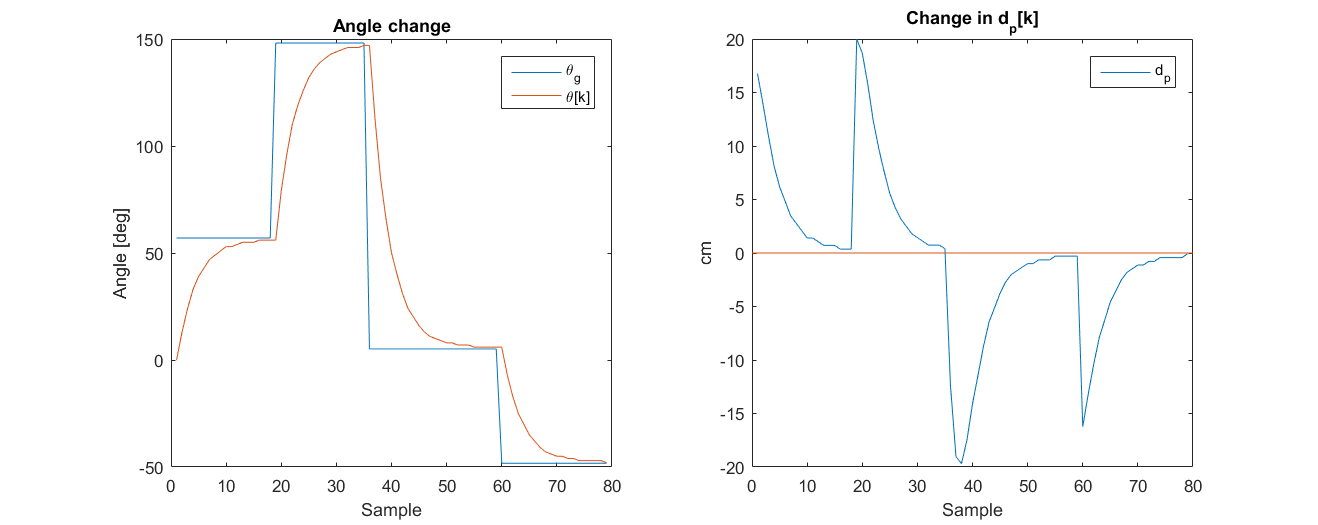
\includegraphics[width=\textwidth]{../matlab/images/task16.png}
  \caption{Control performance when $u_{\omega}=0$}
  \label{fig:task16}
\end{figure}

With the uniform quantizer and samplingtime that we have in our
simulations we get the results presented in figure \ref{fig:task16}. This shows
the control performance for the controller when $u_{\omega}=0$. Since
we cant get the preciseness needed to position the robot we can see that
it will not reach $\theta_g$ exactly but will stop rotating when the
threshold is reached. This is to prevent oscillation around $\theta_g$
which will occur if there is nothing to prevent adjustments when a good
enough presition is reached.
